
\section{Про компьютеры}
\subsection{Транзисторы $\rightarrow$ Процессор}
\begin{frame}[fragile]{Транзисторы $\rightarrow$ Логические элементы}
\begin{itemize}
\item \href{http://www.cs.bu.edu/~best/courses/modules/Transistors2Gates/}{http://www.cs.bu.edu/$\sim$best/courses/modules/Transistors2Gates/}
\item \href{https://www.reddit.com/r/compsci/comments/209fqx/i_want_to_know_how_the_computer_works_from/}{Reddit topic: https://bit.ly/2CdBk3u}
\item \href{https://habr.com/post/338584/}{Реализация «Тетриса» в игре «Жизнь»: https://habr.com/post/338584/}
\end{itemize}
\end{frame}

\begin{frame}[fragile]{Транзисторы $\rightarrow$ Логические элементы}
\begin{multicols}{2}
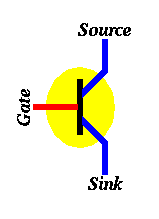
\includegraphics[width=3cm, height=4cm]{Term_1/Source/Pirctures/transistor-n.png}
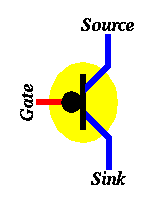
\includegraphics[width=3cm, height=4cm]{Term_1/Source/Pirctures/transistor-p.png}
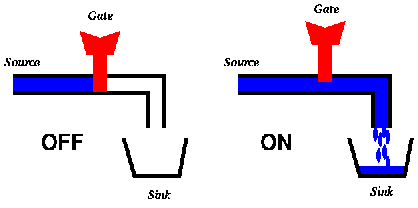
\includegraphics[width=6cm, height=4cm]{Term_1/Source/Pirctures/transistor-as-faucet.png}
\end{multicols}
\end{frame}

\begin{frame}[fragile]{Транзисторы $\rightarrow$ Логические элементы}{NOT}
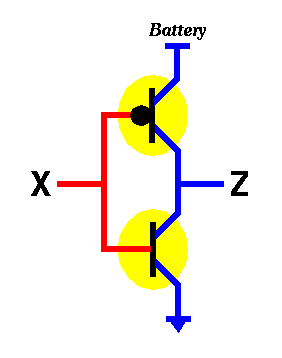
\includegraphics[width=6cm, height=6cm]{Term_1/Source/Pirctures/not-circuit.png}
\end{frame}

\begin{frame}[fragile]{Транзисторы $\rightarrow$ Логические элементы}{NAND}
\begin{multicols}{2}
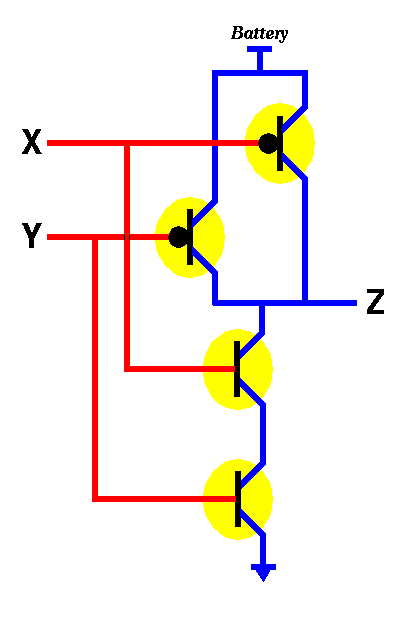
\includegraphics[width=5cm, height=7cm]{Term_1/Source/Pirctures/nand-circuit.png}
\vfill\eject
\begin{tabular}{ c|c|c } 
X &	Y & Z \\ 
  \hline
0 & 0 & 1\\
  \hline
0 & 1 & 1 \\
 \hline
1 & 0 & 1 \\
 \hline
1 & 1 & 0 \\
\end{tabular}
\end{multicols}
\end{frame}

\begin{frame}[fragile]{Транзисторы $\rightarrow$ Логические элементы}{NOR}
\begin{multicols}{2}
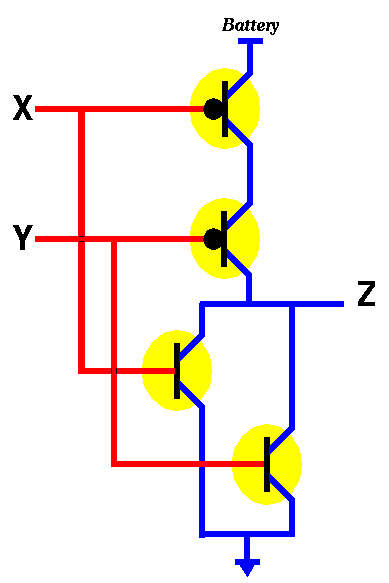
\includegraphics[width=5cm, height=7cm]{Term_1/Source/Pirctures/nor-circuit.png}
\vfill\eject
\begin{tabular}{ c|c|c }
X &	Y & Z \\ 
  \hline
0 & 0 & 1\\
  \hline
0 & 1 & 0 \\
 \hline
1 & 0 & 0 \\
 \hline
1 & 1 & 0 \\
\end{tabular}
\end{multicols}
\end{frame}

\begin{frame}[fragile]{Логические элементы $\rightarrow$ Сумматор}{AND, OR, XOR}
\begin{multicols}{2}
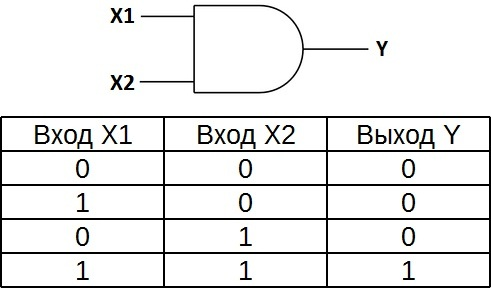
\includegraphics[width=4cm, height=3cm]{Term_1/Source/Pirctures/and.jpg}\\
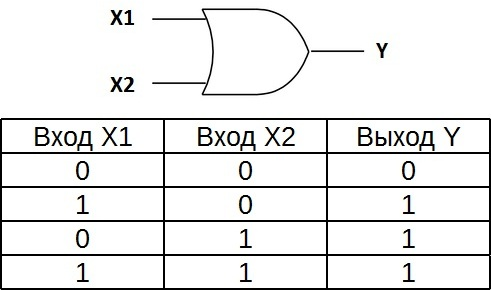
\includegraphics[width=4cm, height=3cm]{Term_1/Source/Pirctures/or.jpg}
\vfill\eject
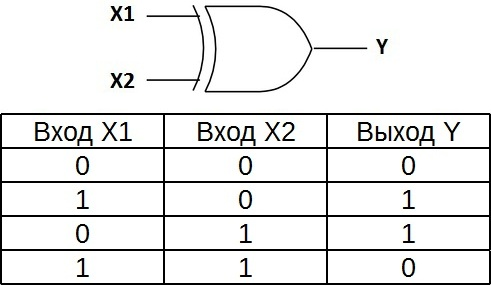
\includegraphics[width=4cm, height=3cm]{Term_1/Source/Pirctures/xor.jpg}
\end{multicols}
\end{frame}


\begin{frame}[fragile]{Логические элементы $\rightarrow$ Сумматор}{Half and full adder}
\begin{multicols}{2}
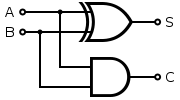
\includegraphics[width=4cm, height=3cm]{Term_1/Source/Pirctures/Half_Adder.png}
\vfill\eject
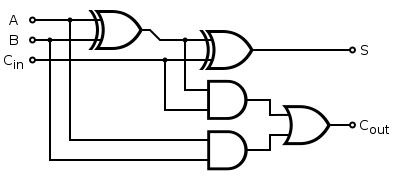
\includegraphics[width=4cm, height=3cm]{Term_1/Source/Pirctures/Full_Adder.png}
\end{multicols}
\end{frame}

\begin{frame}[fragile]{Логические элементы $\rightarrow$ Сумматор}{Линейный каскадный сумматор}
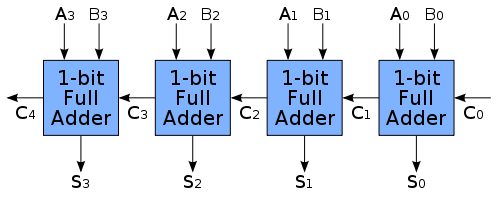
\includegraphics[width=8cm, height=3cm]{Term_1/Source/Pirctures/Ripple_carry_adder.png}
\end{frame}


\subsection{Память}
\begin{frame}[fragile]{Память}
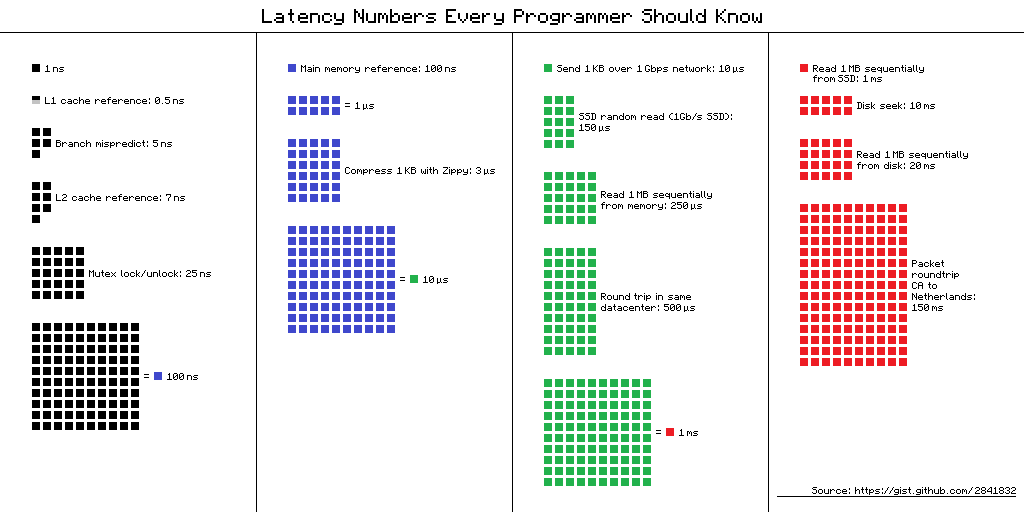
\includegraphics[width=12cm, height=7cm]{Term_1/Source/Pirctures/latency.png}
\end{frame}

\subsection{Архитектура фон Неймана}
\begin{frame}[fragile]{Архитектура фон Неймана}
\begin{itemize}
    \item Работа компьютера контролируется программой, состоящей из набора команд
    \item Принцип последовательного выполнения: после выполнения текущей команды IP (instruction pointer) автоматически указывает на следующую
    \item Принцип однородности: в памяти хранятся и данные, и команды
    \item Принцип адресуемости: память состоит из ячеек, каждая имеет уникальный «адрес»
    \item Использование двоичной системы счисления * (\href{https://habr.com/post/166679/}{https://habr.com/post/166679/})
\end{itemize}
\end{frame}

\begin{frame}[fragile]{Архитектура фон Неймана}
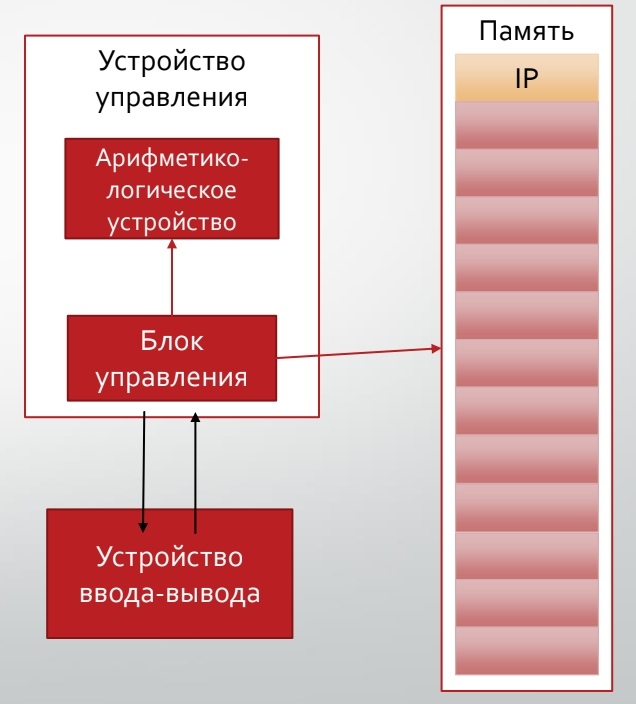
\includegraphics[width=7cm, height=7cm]{Term_1/Source/Pirctures/fon.jpg}
\end{frame}

\begin{frame}[fragile]{Архитектура фон Неймана}
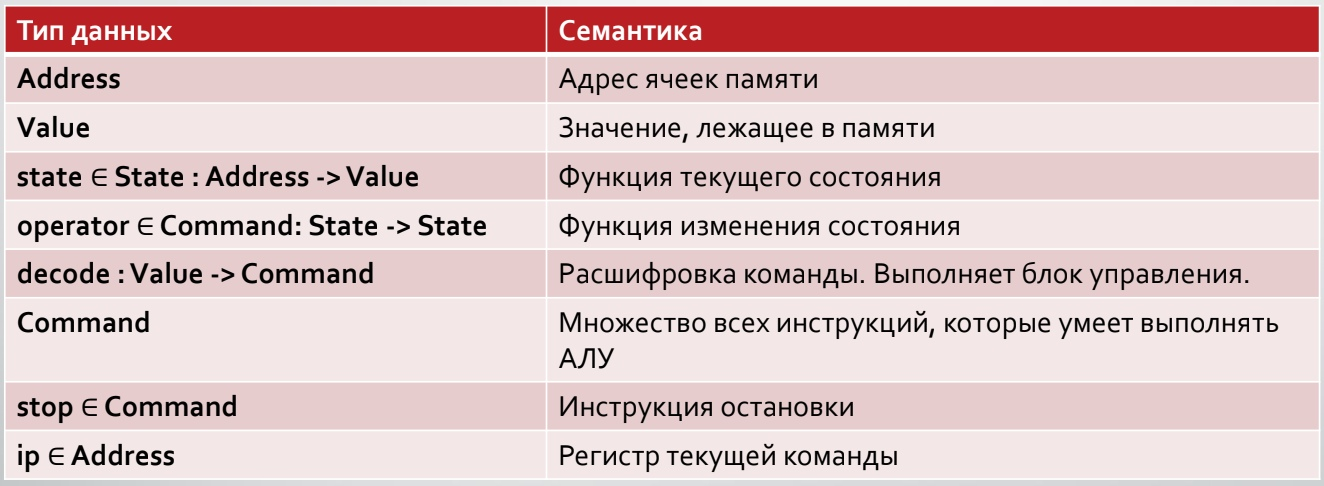
\includegraphics[width=12cm, height=5cm]{Term_1/Source/Pirctures/math-fon.jpg}\\
Принцип хранимой программы: $\forall c \in Command, \exists v \in Value : decode(v) = c $
Текущая операция: $operation = decode(state(state(ip)))$
\end{frame}


\begin{frame}[fragile]{Архитектура фон Неймана}{Пример}
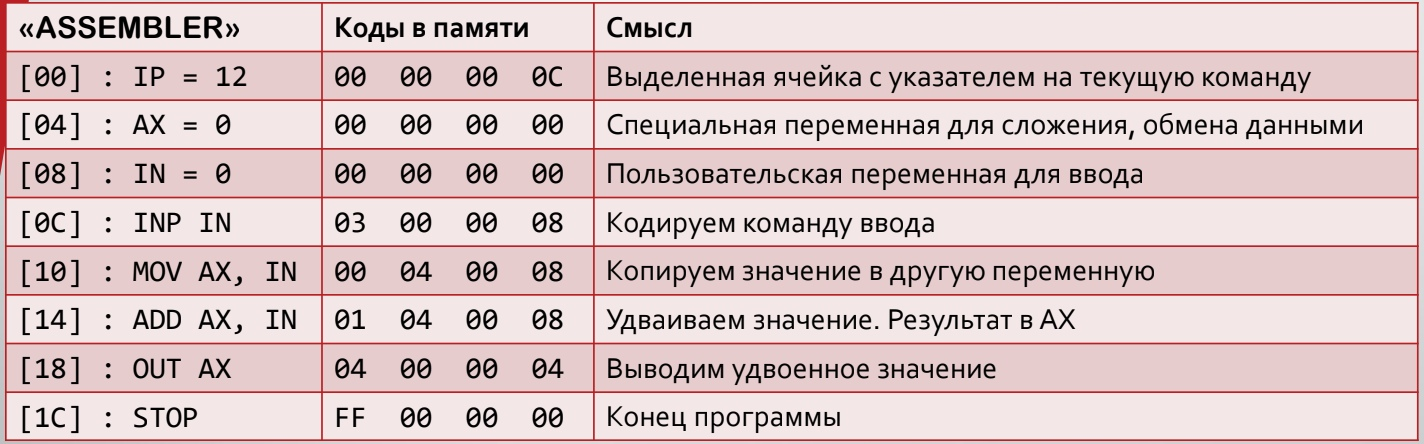
\includegraphics[width=12cm, height=4cm]{Term_1/Source/Pirctures/example.jpg}
\end{frame}

\begin{frame}[fragile]{Архитектура фон Неймана}{Пример}
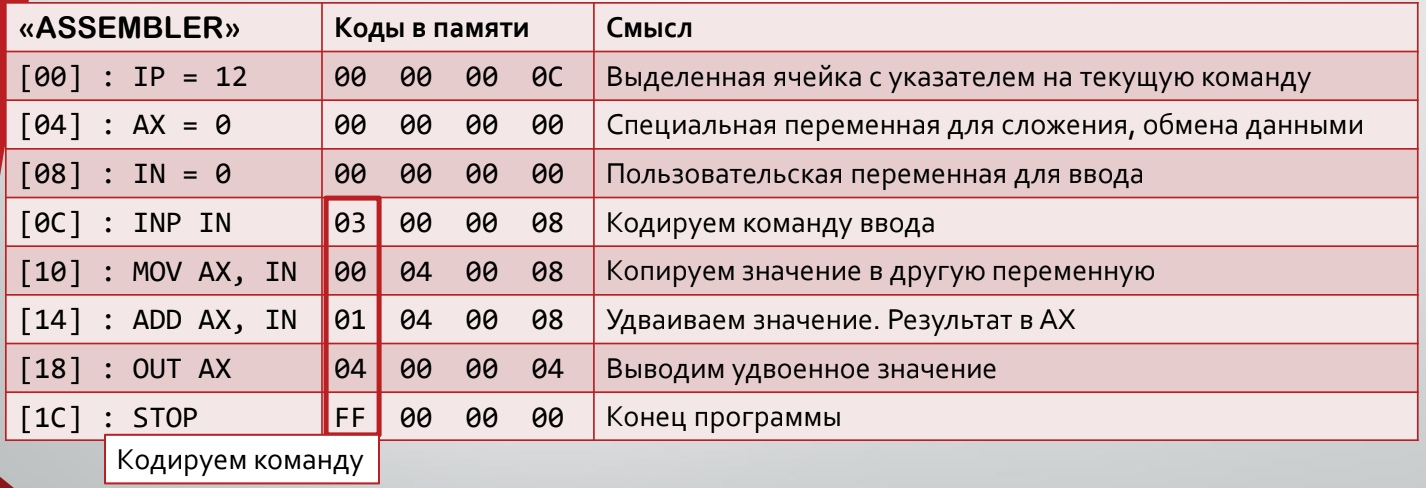
\includegraphics[width=12cm, height=4cm]{Term_1/Source/Pirctures/example1.jpg}
\end{frame}

\begin{frame}[fragile]{Архитектура фон Неймана}{Пример}
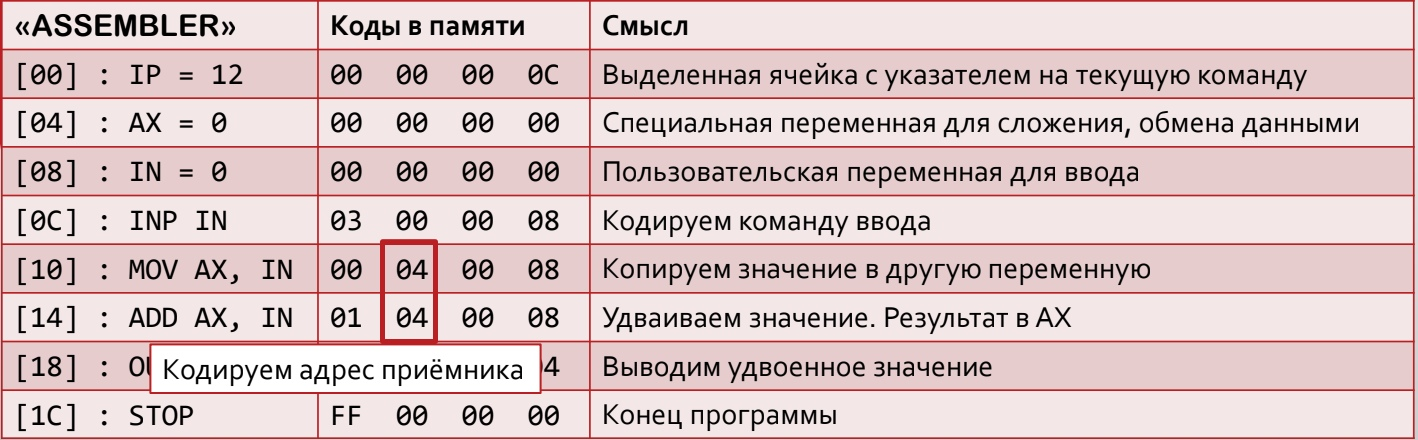
\includegraphics[width=12cm, height=4cm]{Term_1/Source/Pirctures/example2.jpg}
\end{frame}

\begin{frame}[fragile]{Архитектура фон Неймана}{Пример}
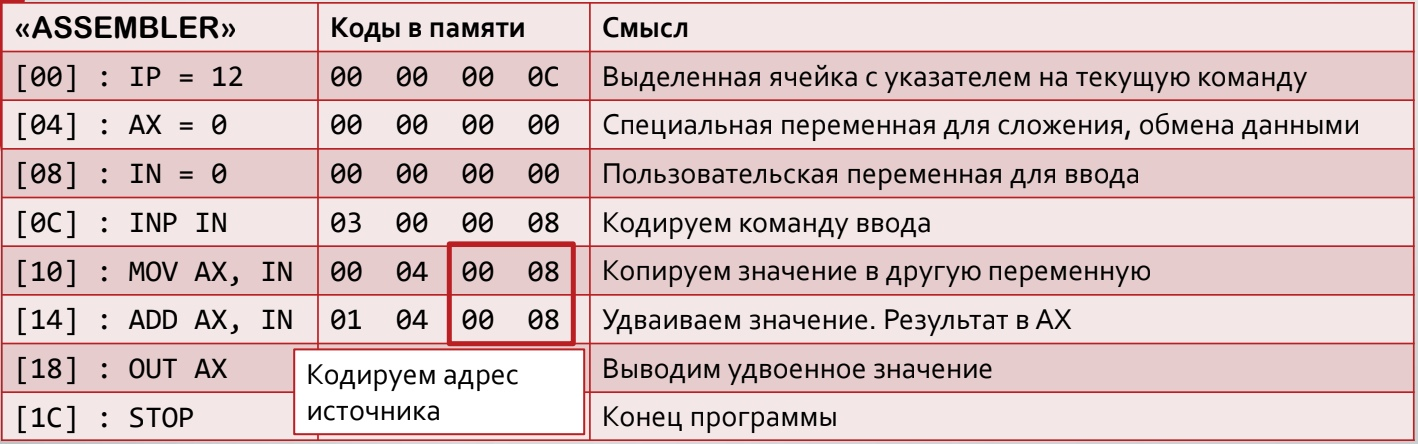
\includegraphics[width=12cm, height=4cm]{Term_1/Source/Pirctures/example3.jpg}
\end{frame}

\begin{frame}[fragile]{Архитектура фон Неймана}{Пример}
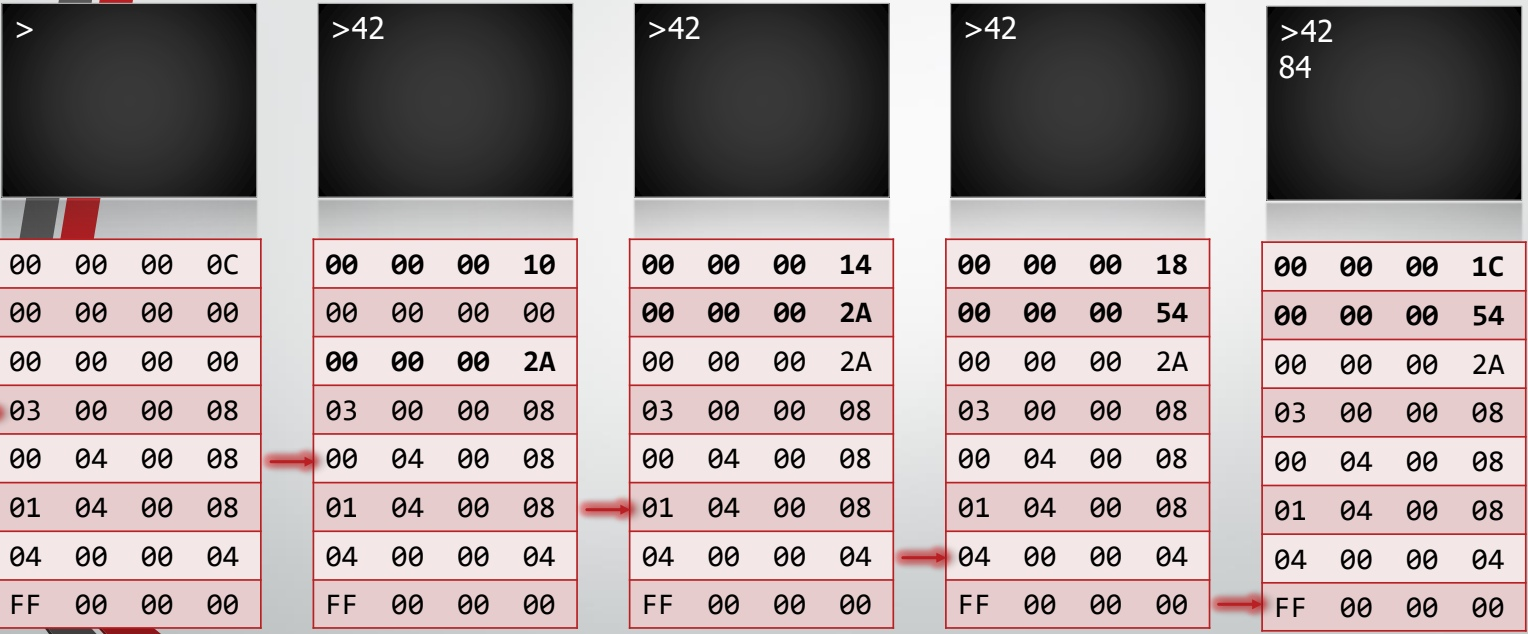
\includegraphics[width=12cm, height=5cm]{Term_1/Source/Pirctures/example-run.jpg}
\end{frame}